%   *******************************************************************
%   * THIS IS THE MAIN FILE--RUNNING LATEX ON "AllegThesis.tex" WILL  *
%   * GENERATE THE ENTIRE THESIS (ASSUMING YOU HAVE NOT RENAMED IT).  *
%   * IF YOU ARE USING BIBTEX, RUNNING BIBTEX ON "AllegThesis" SHOULD *
%   * GENERATE YOUR BIBLIOGRAPHY. SPECIFIC DETAILS DEPEND ON WHAT     *
%   * ENVIRONMENT AND TOOLS YOU ARE USING (E.G., TEXMAKER OR COMMAND  *
%   * LINE TOOLS LIKE PDFLATEX OR ...).                               *
%   *******************************************************************
%
% AllegThesis.tex
% by A. Thall
% 13 Feb 2003
%
% Revised by R. Roos
% Nov 2013
%
% This document provides a sample Senior Thesis template for use
% by students in Allegheny's CS and Applied Computing programs.
%
%   *******************************************************************
%   * LOOK FOR BLOCK COMMENTS SUCH AS THIS ONE FOR AN EXPLANATION OF  *
%   * THIS DOCUMENT AND HOW TO MODIFY IT FOR YOUR OWN THESIS!         *
%   *                                                                 *
%   * ANY LINE BEGINNING WITH A "%" IS A LATEX COMMENT AND IS IGNORED *
%   * BY THE LATEX PROCESSOR. YOU ARE ENCOURAGED TO COMMENT YOUR OWN  *
%   * LATEX CODE TO HELP YOU REMEMBER WHY YOU DID THINGS A CERTAIN WAY*
%   *******************************************************************
%

%   ********************************************************************
%   * THE FIRST SECTION OF THE MAIN LATEX FILE IS THE "PREAMBLE." IT   *
%   * INSTRUCTS LATEX TO IMPORT SPECIAL PACKAGES FOR THINGS LIKE       *
%   * INCLUDING FIGURES, DOUBLE-SPACING, COLORED TEXT, ETC.            *
%   * DEPENDING ON YOUR NEEDS, YOU MAY FIND IT NECESSARY TO USE PACK-  *
%   * AGES THAT ARE NOT INCLUDED IN THIS TEMPLATE. SIMPLY IMITATE THE  *
%   * "\usepackage{...}" COMMANDS SHOWN BELOW.                         *
%   ********************************************************************

%   ********************************************************************
%   * BEGINNING OF PREAMBLE:                                           *
%   ********************************************************************

\NeedsTeXFormat{LaTeX2e}
\documentclass[12pt]{report}

%   ********************************************************************
%   * ALL BUT ONE OF THE FOLLOWING 5 LINES SHOULD BE COMMENTED OUT.    *
%   * (NOT ALL OF THESE OPTIONS HAVE BEEN TESTED IN THIS REVISION!)    *
%   ********************************************************************

%\usepackage[debug,draft,double]{gatorthesis} % for student proof doublespace
%\usepackage[bottom,double]{gatorthesis} % for final department copy
\usepackage[debug,draft,single]{gatorthesis} % for student workcopy
%\usepackage[single]{gatorthesis} % for student
%\usepackage[debug,draft,nolists,nofront,single]{gatorthesis} % more options


\usepackage{comment}     % provides a way to "comment out" sections in blocks
\usepackage{doublespace} % final document should be double-spaced!
\usepackage{amsmath}     % special symbols
\usepackage{amssymb}     % more special symbols
\usepackage{epsfig}      % needed for including figures
% \usepackage{fancybox}  % --- DISABLED BY RSR, SEP 2013 ---
\usepackage{url}
\usepackage{listings}
\usepackage[figure]{algorithm2e}
\usepackage{graphicx}
\usepackage{mathptmx}
\usepackage{fancyhdr}
\usepackage{ragged2e}
\usepackage[T1]{fontenc}
\usepackage{fixltx2e}
\graphicspath{images/}
%   ********************************************************************
%   * OPTIONAL: IF YOU WANT VERY FINE CONTROL OVER HOW LATEX HYPHENATES*
%   * CERTAIN WORDS, YOU CAN PUT WORDS IN A "\hyphenation" COMMAND AS  *
%   * SHOWN IN THE FOLLOWING EXAMPLE. OTHERWISE, YOU MAY JUST IGNORE   *
%   * THE NEXT COMMAND.                                                *
%   ********************************************************************

% EXAMPLE: Don't hyphenate the words "itself" or "linear". Hyphenate 
%          "representations" only at the places indicated by the "-":

\hyphenation{itself repre-sen-tations linear}

%   ********************************************************************
%   * THE FOLLOWING COMMAND HAS BEEN DISABLED--IGNORE.                 *
%   ********************************************************************
% The following provides a box to surround the thesis statement
%\newenvironment{Thesis}%
%{\begin{Sbox}\begin{minipage}{.95\linewidth}}%
%{\end{minipage}\end{Sbox}\begin{center}\fbox{\TheSbox}\end{center}}

%   ********************************************************************
%   ********************************************************************
%   ***  END OF PREAMBLE.                                            ***
%   ********************************************************************
%   ********************************************************************



%   ********************************************************************
%   * DOCUMENT CONTENT STARTS AT THE "\begin{document}" COMMAND:       *
%   ********************************************************************

\begin{document}

%   ********************************************************************
%   * FILL IN THE "{...}" BELOW WITH YOUR INFORMATION.                 *
%   ********************************************************************

\thesistitle{Optimizing Energy Efficiency in Buildings \\using Multi Objective Genetic Algorithms}

\thesisauthor{Dibyajyoti Mukherjee} \thesisadvisor{Dr. Robert Roos}

\thesisnumber{CS14-13} % SEE PAULINE LANZINE TO GET YOUR REPORT NUMBER!

\thesisreadera{Dr. Shaunna Barnhart}


%   ********************************************************************
%   * IN RARE CASES YOU MAY HAVE MORE THAN TWO READERS, IN WHICH CASE  *
%   * YOU SHOULD UN-COMMENT THE FOLLOWING AND ADD NAMES:               *
%   ********************************************************************
% \thesisreaderb{Dr. Your Thirdreader} 
% \thesisreaderc{Dr. Your Fourthreader}
% \thesisreaderd{Dr. Your Fifthreader}

%   ********************************************************************
%   * YOU MAY IGNORE THE FOLLOWING COMMAND:                            *
%   ********************************************************************
\date{\FileRevised \\ $\mbox{}$Revision: 1.8 $\mbox{}$}

\thesismaketitle         % Creates the title page
\thesismakecopyright     % Creates the copyright page

%   ********************************************************************
%   * YOU MAY SPLIT YOUR THESIS INTO SEVERAL FILES AND "\include" THEM *
%   * AS SHOWN BELOW. FOR INSTANCE, FILE "abstract.tex" CONTAINS THE   *
%   * ABSTRACT, FILE "ack.tex" CONTAINS THE ACKNOWLEDGMENTS, ETC. YOU  *
%   * MAY, OF COURSE, PUT EVERYTHING INTO ONE HUGE FILE, BUT THERE ARE *
%   * ADVANTAGES TO SPLITTING THINGS UP--FOR EXAMPLE, YOU CAN COMMENT  *
%   * OUT "\include" LINES OF SOME PARTS IN ORDER TO PRINT DRAFTS      *
%   * CONTAINING SELECTED SECTIONS OF YOUR THESIS, SAVING PAPER AND    *
%   * PRINTING COSTS.                                                  *
%   *                                                                  *
%   * YOU ARE NOT REQUIRED TO HAVE A "dedication"--IF YOU DON'T, JUST  *
%   * DELETE THAT LINE OR COMMENT IT OUT WITH A LEADING "%"            *
%   ********************************************************************

%\begin{abstract}
Using \LaTeX\ to produce a professional-looking senior thesis can
be a daunting task. This work illustrates some of the more common
tools and features of \LaTeX. The PDF version of the thesis, together with
the heavily-commented {\tt .tex} source files used to produce it,
answer many questions commonly asked by
seniors concerning the final typeset thesis document.
\end{abstract}
  % REQUIRED!

%\include{dedication} % OPTIONAL

%\include{ack}       % OPTIONAL, BUT ALMOST EVERYONE INCLUDES IT

%   ********************************************************************
%   * FRONT MATTER--TABLE OF CONTENTS, ETC. YOU PROBABLY DON'T NEED TO *
%   * CHANGE ANY OF THIS UNLESS YOU HAVE NO TABLES OR FIGURES, OR YOU  *
%   * WANT TO CHANGE NUMBERING DEPTH FOR SUBSECTIONS, OR ...           *
%   ********************************************************************

\setcounter{tocdepth}{2}    % # of section levels shown in table of contents
\setcounter{secnumdepth}{3} % # of numbered subsection levels in the text

\tableofcontents
%\listoftables       % OMIT THIS IF YOU DON'T HAVE ANY TABLES
\listoffigures      % OMIT THIS IF YOU DON'T HAVE ANY FIGURES

%   ********************************************************************
%   * A GLOSSARY IS ALMOST NEVER NEEDED UNLESS YOU HAVE AN UNUSUALLY   *
%   * LARGE NUMBER OF SPECIAL TERMS OR NOTATIONS AND IT WOULD DETRACT  *
%   * TOO MUCH FROM THE FLOW OF THE PAPER TO DEFINE THEM IN-LINE.      *
%   ********************************************************************
%\include{glossary}  % OMIT THIS IF YOU DON'T HAVE A GLOSSARY (FEW PEOPLE DO)


%   ********************************************************************
%   * THE FOLLOWING "lstset" COMMAND IS ADAPTED FROM ONE FOUND AT:     *
%   * http://tex.stackexchange.com/questions/115467/                   *
%   * listings-highlight-java-annotations                              *
%   *                                                                  *
%   * SEE CHAPTER 3 AND APPENDIX A                                     *
%   ********************************************************************

\lstset{
  basicstyle=\footnotesize\tt, % the size of the fonts that are used for the code
  breakatwhitespace=false,     % automatic breaks only happen at whitespace?
  breaklines=true,             % sets automatic line breaking
  captionpos=b,                % sets the caption-position to bottom
  frame=single,                % adds a frame around the code
  language=Java,               % the language of the code
  keywordstyle=\bf,
  showspaces=false,
  showstringspaces=false,      % underline spaces within strings only?
  showtabs=false,
  tabsize=2                    % sets default tabsize to 2 spaces
}

%   ********************************************************************
%   * NOW INCLUDE THE CHAPTER FILES; COMMENT OUT ANY YOU DON'T WANT TO *
%   * PROCESS IN A PARTICULAR LATEX RUN.                               *
%   *                                                                  *
%   * INCLUDED FILES ARE ASSUMED TO END IN ".tex", E.G.,               *
%   * "ch01_overview.tex", "ch02_relatedwork.tex", ETC.                *
%   ********************************************************************

% ch:intro
%
% $Id: ch01_overview
%
%   *******************************************************************
%   * SEE THE MAIN FILE "AllegThesis.tex" FOR MORE INFORMATION.       *
%   *******************************************************************

\chapter{Introduction}\label{ch:intro} % we can refer to chapter by the label

%   ************************************************************************
%   * In LaTeX, new paragraphs are begun by simply leaving a blank line in *
%   * the LaTeX file.                                                      *
%   *                                                                      *
%   * The \\ characters should NEVER be used to end a paragraph.           *
%   * They are used only for inserting line breaks in certain situations.  *
%   *                                                                      *
%   * "Widows" (ending paragraph lines at the top of a new page) and       *
%   * "orphans" (opening paragraph lines at the bottom of a page) should   *
%   * be eliminated; this sometimes requires re-writing some of the        *
%   * text to change the line lengths.                                     *
%   ************************************************************************


\section{Importance of Energy Efficiency} \label{sec:motivation}

Energy usage globally has risen about 70 percent since 1971 and is projected to continue to rise in the future as countries across the world become more developed and have larger economies. Based on 2010 estimates, energy demand is projected to rise at over 2 per cent per year for the next 15 years if current energy usage patterns persist \cite{wri}. Rising energy use leads to an increase in greenhouse gas emissions from fossil fuels which further leads to an increase in chances of climate change. According to the World Resources Institute, about 90 percent of the world's commercial energy comes from fossil fuels, and ``energy related emissions account for more than 80 percent of the carbon dioxide (CO\textsubscript{2}) released into the atmosphere each year'' \cite{wri}. Global energy consumption and annual CO\textsubscript{2} emissions have risen by almost 50 percent from 1993 levels \cite{wri}.

Energy efficiency, i.e., delivering the same (or more) services for less energy, is one of the quickest and cheapest ways to increase the amount of energy available for use. The European Council for an Energy Efficient Economy describes energy efficiency  as the `cornerstone of a sustainable society' \cite{ecees}.A large share of the energy supply has to come from renewable energy sources such as wind and solar power in order to comply with international treaties such as the Kyoto Protocol. However, with increasing energy demand, the development of renewables needs to be supplemented with energy efficiency.

From an environmental perspective, an obvious benefit to energy efficiency is 
the reduction in the amount of greenhouse gas emissions. Reduction in greenhouse gas emissions can help with  improving urban air quality, reducing acid rain, and reducing eutrophication (i.e. an increase in the concentration of nutrients in water that promotes excessive algae growth) \cite{ecees}. There are economic benefits to energy efficiency as well. According to the Department of Energy's Energy Efficiency and Renewable Energy program, Americans saved \$7 billion on residential energy bills in 2004 from energy saving measures and by building energy efficient homes \cite{wri}. Increased energy efficiency contributes to energy security and makes a country more competitive in an increasingly globalized world. 

Buildings have an enormous impact on the environment, using about 40 percent of natural resources extracted in industrialized countries, consuming nearly 70 percent of electricity and 12 percent of potable water, and producing between 45 and 65 percent of the waste disposed in landfills. Moreover, they are responsible for a large amount of harmful emissions, accounting for 30 percent of greenhouse gases, due to their operation, and an additional 18 percent caused indirectly by material exploitation and transportation \cite{Castro-Lacouture2009}. Buildings in the United States account for about 39 percent of the total primary energy consumption and 70 percent of the electricity consumption(Fig.\ref{fig:energy})\cite{Wang2005a}. Energy efficiency in buildings can thus play an important role in making the building `green'. Some such measures are structural and can only be included in newly constructed buildings; many others can be incorporated during building refurbishment. While there are software tools available to simulate the effects and impacts of a particular design, tools for optimizing the design are not readily available \cite{Wang2005b} \cite{Pernodet2009}.

\begin{figure}[htbp]
\centering
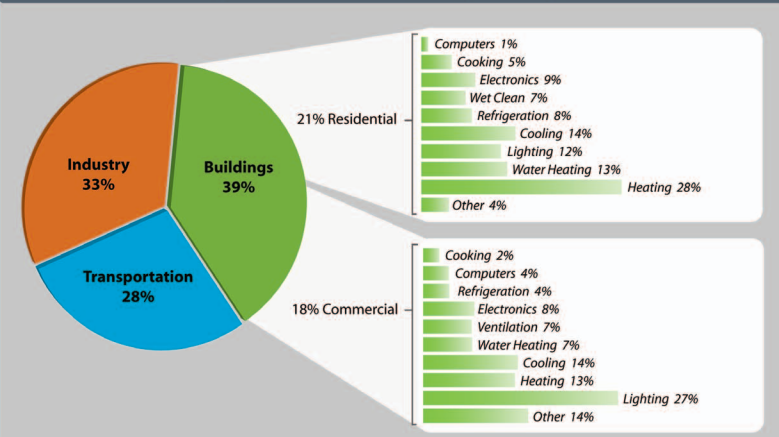
\includegraphics[width=0.8\linewidth,scale=0.6]{images/energy.png}
\caption{Buildings Share of U.S. Primary Energy Consumption 
Uses \cite{wri}}
\label{fig:energy}
\end{figure}

\section{Optimization techniques}\label{sec:stateofart}
Solving an optimization problem allows us to find at least one solution that 
minimizes or maximizes a particular criterion. This criterion is represented by an objective or a fitness function that depends on variable parameters (both continuous and discrete) that describe the solutions \cite{Pernodet2009}. 
Optimizations can be both single criterion or multi criteria. There are three 
main methods for optimization: enumerative, calculus based, and random \cite{Pernodet2009}. Enumerative methods go through every single solution in the search space in order to find the optimal one. While this method is simple, it is extremely inefficient especially when it comes to problems such as building optimization due to the huge number of possible solutions. Calculus based methods use a rigorous mathematical expression of the objective function. The main limitation to this method, besides having to know an explicit mathematical expression (that sometimes has to be continuous), is that it can find a local optimum in the neighborhood without going through the global search space. Random methods, as the name suggests, use random evaluation of solutions and are often built to emulate other phenomena.

\begin{figure}[htbp]
\centering
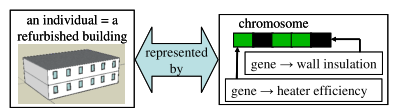
\includegraphics[width =0.7\linewidth]{images/pernodet.png}
\caption{Representing solutions as chromosome \cite{Pernodet2009}}
\label{fig:pernodet}
\end{figure}


Genetic algorithms (GAs) are a form of random optimization methods that seek to mimic the process of evolution in order to select an optimal solution. Strings of either real numbers or  bits (binary digits, 0 and 1) are used analogous to a gene in order to represent the parameters (Fig.\ref{fig:pernodet}) \cite{Pernodet2009} \cite{Coley2002}. Multiple such sub-strings are then concatenated to form the genotype. An initial population of theses genotypes is generated randomly. The algorithm consists of three main functions : selection, mutation and crossover (Fig.\ref{fig:pernodet2}). During selection, the fitness of an individual string is evaluated using the parameter values it represents. The fittest of the strings are then crossed-over i.e. allowed to mate and produce progeny by combining substrings of random length from pairs of genotypes. Mutation is allowed by occasional changing the values of a string position of a newly created progeny. After a number of generations of the process, the parameter values represented by the genotypes hopefully converge towards optimal solution values \cite{Coley2002}.

\begin{figure}[htbp]
\centering
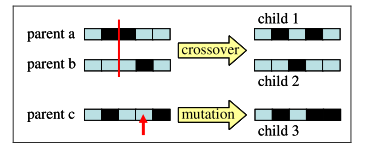
\includegraphics[width =0.7\linewidth]{images/pernodet2.png}
\caption{Crossover and Mutation operators \cite{Pernodet2009}}
\label{fig:pernodet2}
\end{figure}


The general advantages of using genetic algorithms for optimization problems are all relevant in the case of energy optimization for buildings. GAs do not 
require a knowledge of the mathematical structure of the problem. A GA search is not limited to a local optimum \cite{Pernodet2009}. Further, multi objective GAs such as the non-dominated sorting genetic algorithm (NSGA-II) produce Pareto optimal solutions. A solution is Pareto optimal if a decrease in one objective cannot happen without an increase in at least one other objective \cite{Deb2002}\cite{Pernodet2009}. For a problem with two objectives (such as energy consumption and cost), the result is a curve of Pareto solutions instead of just one solution. Thus, this allows us to obtain a whole set of solutions from which we can then choose (Fig.\ref{fig:pareto}). %Add more about MOGA%

\begin{figure}[htbp]
\centering
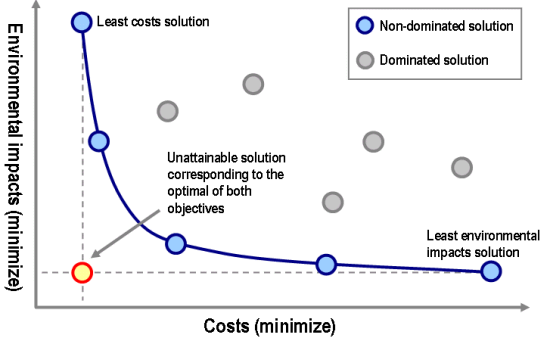
\includegraphics[width = 0.5\linewidth]{images/pareto.png}
\caption{Pareto Optimal Solution Curve \cite{Coley2002}}
\label{fig:pareto}
\end{figure}

\section{Goals of the Project}\label{sec:goals}

The aim of this proposed project is to use a genetic algorithm based approach 
to create a system for optimizing energy efficiency in a building. The system 
will take in parameters needed to model the building design and output a set of Pareto optimal solutions. This will be a multi-objective optimization problem with two objectives\textemdash minimizing energy usage and minimizing associated cost. A multi-objective genetic algorithm, NSGA-II will be used along with a building energy simulation program, EnergyPlus for fitness evaluation. The following chapters outline genetic algorithm and the NSGA-II algorithm in details, discuss some related work in the field and explain the method of approach. I will also present the results of a case study of the system using Alden Hall, a building on Allegheny College campus. Finally, I will discuss the results of the case study in context of other related work in the area.


% COMMENTED OUT NEXT FEW LINES TO SAVE SPACE; MAY PUT THEM BACK LATER
%Following the concise statement of the thesis, some of the details can be
%expanded.  
%It is appropriate to
%refer to some of the results in the introduction (which may 
%mean going back and adding them to the introduction once the
%research is completed). 
%A senior thesis, or any research paper, is not a mystery 
%novel---there is no need to keep the reader in suspense about what
%has been accomplished.

% \section{Thesis Outline}\label{sec:outline}
% The introductory chapter usually concludes with a ``road map'' of the upcoming
% chapters, e.g., ``Chapter \ref{ch:relatedwork} reviews a number of past approaches
% to the problem and summarizes their strengths and weaknesses. Chapter 
% \ref{ch:method} outlines the method of approach used to establish the
% results.''
 % Introduction -- of course, you can name it anything!

% ch:relatedwork
%
% $Id: ch02_relatedwork
%
%   *******************************************************************
%   * SEE THE MAIN FILE "AllegThesis.tex" FOR MORE INFORMATION.       *
%   *******************************************************************
\chapter{Related Work}\label{ch:relatedwork}

Genetic algorithms have been used to solve optimization problems for new buildings as well as for refurbished buildings. While some studies have focused on energy efficiency, others have included other factors such as material selection and structural design  \cite{Castro-Lacouture2009} \cite{Behboudi2012}. In this chapter, I will analyze four different studies involving building optimization using genetic algorithms. These five studies have significant differences in their goals and depth, thereby providing a broad overview of the topic. I will mainly concentrate on how the authors formulated the objective functions, what variables they used in the genetic algorithm, and how they implemented their system.

\section{Objective Functions}\label{sec:functions}

Wang et al. present a case study that uses their multi-objective framework to design a single story office building in Montreal, Canada \cite{Wang2005b}. The objective functions they use are the total life cycle cost and life cycle environmental impact for a green building design. They use exergy, i.e., the maximum theoretical work that can be done by a system with respect to its environment, as the indicator for environmental impacts \cite{Wang2005b}. Besides the exergy consumed by the building during its lifecycle, they also consider the exergy required to remove or recover the wastes produced in the different life cycle phases of the building such as greenhouse gases \cite{Wang2005b}. For the cost objective, they consider the inital construction cost, the operation cost, and the pre-operation cost including resource extraction, transportation, etc. \cite{Wang2005b}. 

Milajec et al. use similar objective functions as Wang et al. i.e. life cycle cost and life cycle environmental impact. While they do include both cost of construction and of operation, they do not specify whether they include pre-construction cost as well. Their life cycle environmental impact assesment cost includes the cumulative exergy (like Wang et al.) but not the exergy required for waste recovery or removal. The Pernodet et al. study uses some similar objective functions as well. The main difference is that instead of two they use three objective functions \textemdash yearly energy consumption of the building in KwH/m\textsuperscript{2}, investment cost related to the refurbishment of the building, and an economic global cost defined as the ``sum of initial investment cost, the yearly energy cost and the yearly maintenance cost'' \cite{Pernodet2009}. Their study looks at optimizing the refurbishment of a school building in France.

Unlike the above studies, Magnier et al. and Pejicic et al. do not use cost as an objective function. Magnier et al. focus on thermal comfort as an objective function aside from energy consumption. Pejicic et al. use a case study to demonstrate multi objective optimization using a model single floor commercial building. Their goal is the optimization of insulation materials and orientation angle of a given building. 


\section{Building variables}\label{sec:variables}

Pejicic et al consider three building variables in their studies \textemdash building orientation, and inner and outer insulation materials from a set of ten different materials. Pernodet et al. \cite{Pernodet2009} focus on the building envelope parameters for their objective function. These include thermal transmittance of the walls and windows, glazing ratio and solar factor, air tightness of building envelope, and artificial lighting power. Similarly, Milajec et al. mainly consider structural variables as well incluidng wall, floor, and roof type and layers, building shape, orientation and structure. The Wang et al. study is much more in depth as they consider the most variables out of any of the above studies. Further, many of their variables are composed of other sub-variables. For instance, they have two different wall types and each wall type has a sub-variable called insulation among other ones. Insulation is a discrete variable that can take many different values, each corresponding to a different insulation material. Each wall type has a specific set of insulation materials to choose from. Besides wall type, Wang et al look at floor types, roof type, and building shape. Each of these has its own set of sub-variables making the Wang study significantly more complex than the others. While the above studies consider only variables related to the building envelope, Magnier et al. use HVAC system-related variables in addition to the building envelope ones. They use a total of 20 different variables including heating and cooling set points, relative humidity set point, supply air flow rates, thermostat delays, window sizes, thickness of wall etc. The window sizes are separate for each wall and the HVAC system related variables are considered separately for two different seasons in a year. 


\begin{figure}[htbp]
\centering
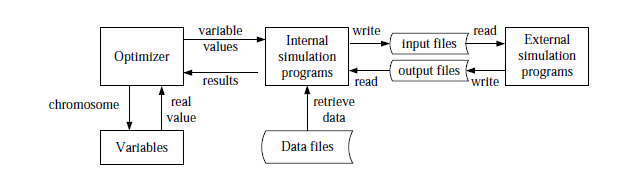
\includegraphics[width=\linewidth]{images/ooframework.png}
\caption{Object Oriented Framework used by Wang et al. \cite{Wang2005b}}
\label{fig:wang}
\end{figure}

\section{Implementation}\label{sec:implementation}
 Wang et al. \cite{Wang2005b} present an extensible object oriented framework implemented in C++ and Fortran (Fig. \ref{fig:wang}). The object oriented nature of the framework presented makes it easily extensible and promotes code reuse. The framework supports both continuous and discrete variables and implements algorithms to solve both unconstrained and constrained single objective optimization problems, but only unconstrained multi-objective optimization problems. Constrained, as the name suggests, limits the range of values for a variable to certain range as specified by the user while unconstrained does not. The framework integrates with the commercially available ASHRAE Toolkit energy simulator program and can be extended to integrate with {\em EnergyPlus}. The authors use the framework for a case study with impressive results and present a number of ways in which the project can be extended. While this framework can certainly be very useful as a starting base for my proposed project, it is not readily available as a open source project. 

Unlike Wang, other studies focus less on the software framework and more on the method of approach of completing the optimization process. Indeed, Pejicic et al. state that a ``solving methodology using evolutionary algoritms'' as their objective. A major difference in implentation between the Wang et al. study and the others is the energy simulation software used \textemdash both Milajec et al. and Pejicic et al. use EnergyPlus while Magnier et al. use TRYNSYS.  While TRYNSYS is widely used in industry (CITE), EnergyPlus is newer and cross-platform, and is freely available from the Department of Energy. In addition, it supports modelling a building through Sketchup through a free plugin. The ASHRAE Toolkit is older than EnergyPlus and does not support as many thermal modelling options either. Pernodet et al. do not use thermal simuation at all. Instead they estimate energy usage mathematically. This method is simple though it might be inaccurate for more complex buildings.

One of the main drawbacks of using an energy simulation program is that they are time consuming. Wang et al. report that a complete optimization run for their case study took about 70 hours. EnergyPlus and TRYNSYS would be even slower since their thermal simulation model is more complex. To counter this problem, Magnier et al. use an artificial neural netowrk (ANN) for fast evaluation. They use a multilayer feed-forward ANN to first mimic the behavior of the base building model, and then use this ANN inside the GA for fast evaluation of individuals (Fig. \ref{fig:magnier}). This technique is very efficient and reduces the computational time associated with each evaluation to almost negligible while maintaining a good accuracy \cite{Magnier2010}. The main limitation to this method is that the ANN needs to be trained before it can be used for the evaluations. The training period can take a relatively large amount of time. For instance, the training period in the Magnier et al. study was around 3 weeks. The advantage, however, is that the once the ANN is trained, it can be used for multiple runs of the system. A different approach would be to use a distributed model of computing by dividing the task of evaluating the fitness of an individual among a cluster of computers instead of a single one. While this method has not been used for optimizing building design in particular, it has been used for other similar multi-objective optimizaton problems. 


\begin{figure}[htbp]
\centering
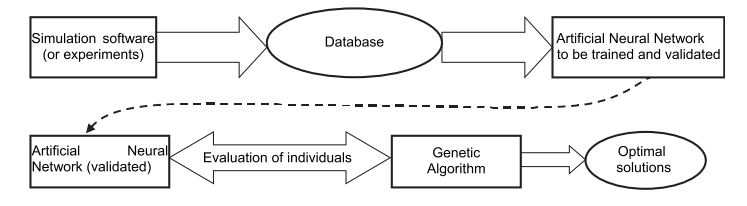
\includegraphics[width = \linewidth]{images/magnier.png}
\caption{Optimization system used by Magnier et al. \cite{Magnier2010}}
\label{fig:magnier}
\end{figure}



 % Background, literature survey, ...

% ch:method
%
% $Id: ch03_thework.tex
%
%   *******************************************************************
%   * SEE THE MAIN FILE "AllegThesis.tex" FOR MORE INFORMATION.       *
%   *******************************************************************
%
\chapter{Implementing the System} \label{ch:method}
The system is implemented using version 7 of the Java programming language using version 21 of the Evolutionary Computation for Java (ECJ) framework. \textit{EnergyPlus} version 8.1 is used for simulating energy usage of the buildings. The implementation was done on Mac OSX 10.9 and Debian Linux version 7.0 running on the Google Compute Engine cloud platform.

\section{Formulating the system}

The two objective functions are:
\begin{itemize}
\item Minimizing the total energy usage. This includes the total electricity usage for a year as well as energy used for heating.
\item Minimizing the associated lifecycle cost. This includes the costs associated with making construction (i.e. material and labor costs) as well as the cost of operation.

\begin{table}[htbp]
    \centering
    \begin{tabular}{|l|l|l|}
    \hline
    Variable name                  & Type       & Unit                      \\ \hline
    Window glazing Material        & Discrete   & N/A                      \\
    R Value of Insulation Material & Discrete   & m\textsuperscript{2}K/W   \\ \hline
    \end{tabular}
    \caption{Building envelope variables }
    \label{table:envelope}
\end{table}

\end{itemize}

There are 5 different building variables that comprise the chromosome for an individual building in the system. These can be classified into two main categories\textemdash building envelope related, and HVAC system related. Building envelope system related variable include window glazing material, window sizes, and insulation material used (Table. \ref{table:envelope}). Glazing type is chosen from a set from the set of five commonly used types as specified by the Energy Information Administration (Table. \ref{table:glazing}). All insulation materials that come bundled with \textit{EnergyPlus} are supported. The costs are determined using data from the Energy Information Administration \cite{eia}. The HVAC system related variables include the HVAC system type (Table. \ref{table:havc_type}), and heating and cooling set points (Table. \ref{table:hvac}).

\begin{table}[htbp]
    \centering
    \begin{tabular}{|l|}
    \hline
    Glazing Type             \\ \hline
    Gas-fills                 \\
    Heat absorbing             \\
    Low emissivity coatings     \\
    Reflexive coatings           \\
    Spectrally selective coatings \\ \hline
    \end{tabular}
    \caption{Glazing type for windows}
    \label{table:glazing}
\end{table}


The building variables were chosen on the basis of a number of factors. First, they had to be supported by \textit{EnergyPlus} as otherwise their effect cannot be quantized during fitness evaluation. Next, the variables had to serve a practical purpose. For instance, while building orientation and shape can influence energy efficiency, it is unlikely that they can be changed (unless one is designing a new building from scratch). Similarly, \textit{EnergyPlus} supports district heating as a HVAC system type. However, it is not feasible to implement such as system since they are implemented on a community scale. Finally, the variables had to have been used in a recent related work and have had a non-negligible impact in the results of those studies. Magnier et al. \cite{Magnier2010} have used heating and cooling set points as well as window glazing materials while Peji\v{c}i\'{c} et al. \cite{Pejicic2012} have used insulation materials for walls. While the type of HVAC system has not been used in any of these studies, my hypothesis is that switching to more efficient HVAC systems will have a significant change in the overall energy use of a building.

\begin{table}[htbp]
    \centering
    \begin{tabular}{|l|l|l|}
    \hline
    Variable name                  & Type       & Unit                      \\ \hline
    Heating Set Point              & Continuous & $^{\circ}$C                       \\
    Cooling Set Point              & Continuous & $^{\circ}$C                       \\
    HVAC System Type               & Discrete   & N/A                        \\ \hline
    \end{tabular}
    \caption{HVAC System variables }
    \label{table:hvac}
\end{table}

%Table for insulation materials

\begin{table}[htbp]
    \centering
    \begin{tabular}{|l|}
    \hline
    Name                \\ \hline
    Furnace             \\
    Heat Pump            \\
    Central Boiler        \\
    Packaged Unit          \\ \hline
    \end{tabular}
    \caption{HVAC System Types}
    \label{table:havc_type}
\end{table}


% \begin{algorithm}[htbp]
%  %\SetLine % For v3.9
%  \SetAlgoLined % For previous releases [?]
%  \KwData{this text}
%  \KwResult{how to write algorithm with \LaTeX2e }
%  initialization\;
%  \While{not at end of this document}{
%   read current\;
%   \eIf{understand}{
%    go to next section\;
%    current section becomes this one\;
%    }{
%    go back to the beginning of current section\;
%   }
%  }
%  \caption{How to write algorithms (from \cite{Fiori:2013})}
% \label{widgmin}
% \end{algorithm}

\section{Fitness Evaluation using {\it EnergyPlus}}

Energy simulation for the building is a central part of the fitness evaluation. \textit{EnergyPlus} is a building energy simulation program developed by the US Department of Energy (DOE) that can be used for energy analysis and building load simulation. According to the product website \cite{eplus}:
\begin{quote}
Based on a user's description of a building from the perspective of the building's physical make-up and associated mechanical and other systems, \textit{EnergyPlus} calculates heating and cooling loads necessary to maintain thermal control set points, conditions throughout a secondary HVAC system and coil loads, and the energy consumption of primary plant equipment. 
\end{quote}
\textit{EnergyPlus} version 8.0 is used in the project for running annual energy simulation for each individual building in a population. The simulation is run using a time step of 15 minutes as this is the minimum that the \textit{EnergyPlus} documentation recommends. \textit{EnergyPlus}, by default, is a command line based program that uses a text based IDF file for input and can produce output in many different formats including HTML and CSV. A number of plugins are also available that add a graphical user interface.

Initially the building to be optimized is modeled in OpenStudio, a free plugin for \textit{EnergyPlus} with a graphical user interface. The resulting text based IDF file is modified by ECJ during runtime and used by \textit{EnergyPlus} to run the simulations. The output is produced in the form of a comma separated value (CSV) file that lists the annual as well as monthly energy and electricity consumption in Joules. This information is used by ECJ to determine the fitness value for the individual building. A single building simulation in \textit{EnergyPlus} can take between 15 seconds to more than a minute. The difference is a result of the complexity of the building design being used. A sample simulation building with  3 floors divided into 3 zones with a fully configured HVAC system as well as solar panels took 70 seconds to run. Using this time as an average, an optimization using a population of 20 and 100 generations would take approximately 39 hours to run.

\section{Extending ECJ}

The ECJ implementation of the NSGA-II algorithm as well as that of the selection, mutation, and crossover operations are used in the system. Individuals are represented using ECJ's \texttt{DoubleVectorIndividual} as arrays of \texttt{double}s. The population size, number of generations, crossover and mutation types can be specified using a text based parameter file (\ref{table:params}). The range for each building variable (gene) can also be specified using the parameter file. 

\begin{table}[htbp]
    \centering
    \begin{tabular}{|l|l|}
    \hline
    Parameter Name                 & Values  \\ \hline
    Population size                & Integer Value (usually between 50 and 100) \\
    Number of generations          & Integer Value \\
    Crossover type                 & One point, Two point, Simulated binary, or Uniform \\ 
    Mutation type                  & Uniform, Gaussian, or Polynomial \\
    Selection type                 & Tournament, Roulette, Random, or Best \\ \hline
    \end{tabular}
    \caption{Genetic Algorithm Parameters supported by the system}
    \label{table:params}
\end{table}

A custom fitness evaluation method was created by implementing the \\
\texttt{ec.simple.SimpleProblemForm} interface and extending the \texttt{ec.Problem} class. The \texttt{evaluate} method in this class reads in an \texttt{Individual} among other parameters. The genome for the \texttt{Individual} is used to modify the input file for \textit{EnergyPlus}. The modified input file is then used to run the annual energy usage simulation for the building. The output from the simulation i.e. the total electricity and the total energy from natural gas is used to assign the fitness value for each objective. The energy usage objective is assigned the total energy usage for the year. The associated cost is calculated by multiplying the electricity and natural gas usage numbers by their respective rates. The rates are assigned from the data provided by the Energy Information Administration \cite{eia}. 

The fitness evaluation is carried out in parallel using ECJ's in-built distributed master slave evaluation model from the \texttt{ec.eval} package. This model consists of one master node along with a number of slave nodes. The master node handles the evolutionary process and sends the individuals to be evaluated at the various slave nodes. As with the rest of the system, the parameters for this module is also specified in a parameter file. These parameters include the IP address for the master node, the number of jobs to be shipped to a slave at once, the number of jobs per slave among others as shown in Table \ref{table:dist_param}. Currently, the system is set up on f1-micro instances of the Google Compute Engine cloud platform. There are 12 slave nodes and 1 master node all running Debian Linux version 7.0. This can easily be changed to any other network by just modifying the IP addresses in the parameters file.

\begin{table}[htbp]
    \centering
    \begin{tabular}{|l|}
    \hline
    Parameter Name                  \\ \hline
    Master IP address               \\
    Master port number               \\
    Job size for shipping             \\
    Number of jobs per slave           \\
    Slave name              \\ \hline
    \end{tabular}
    \caption{Parameters for distributed evaluation}
    \label{table:dist_param}
\end{table}


 % Chapter organization is topic-dependent

%ch:implem
%\include{ch04_implementation} % Chapter organization is topic-dependent

% YOU MAY HAVE SEVERAL MORE CHAPTERS, DEPENDING ON TOPIC AND ORGANIZATION

%ch:conclusion
%%
% $Id: conclusion.tex
%
%   *******************************************************************
%   * SEE THE MAIN FILE "AllegThesis.tex" FOR MORE INFORMATION.       *
%   *******************************************************************
%

\chapter{Conclusion}\label{ch:conclusion}

\section{Summary of Results}

\section{Threats to validity}

\section{Future Work}

 % Conclusion/future work

%   ********************************************************************
%   * IF YOU HAVE ANY APPENDICES (FOR INSTANCE, CODE, DATA, GRAPHS,    *
%   * OR ANYTHING ELSE THAT DOESN'T "FIT" AS REGULAR CHAPTER CONTENT), *
%   * INCLUDE THE FOLLOWING LINE, WHICH INSTRUCTS LATEX TO CHANGE FROM *
%   * NUMBERED "CHAPTER" HEADINGS TO LETTERED "APPENDIX" HEADINGS.     *
%   *                                                                  *
%   * APPENDICES HAVE THE SAME FORMATTING COMMANDS AS CHAPTERS (E.G.,  *
%   * "\chapter{...}", "\section{...}", ETC.)                          *
%   ********************************************************************

\appendix

%%
% $Id: appa--code
%
%   *******************************************************************
%   * SEE THE MAIN FILE "AllegThesis.tex" FOR MORE INFORMATION.       *
%   *******************************************************************

\chapter{Java Code}\label{appa:code}
All program code should be fully commented. Authorship
of all parts of the code should be clearly specified. 

%   *******************************************************************
%   * SEE THE MAIN FILE "AllegThesis.tex" FOR THE "\lstset" COMMAND   *
%   * THAT DEFINES HOW PROGRAM LISTINGS WILL LOOK.                    *
%   *******************************************************************

\lstinputlisting{SampleProg.java}

  % Appendices go here

%   ********************************************************************
%   * THE FINAL COMMANDS DEAL WITH BIBLIOGRAPHY/REFERENCES. IF THERE   *
%   * ARE ANY ITEMS IN YOUR BIBTEX FILE THAT YOU DID NOT REFERENCE IN  *
%   * YOUR PAPER, BUT THAT YOU WISH TO INCLUDE IN THE BIBLIOGRAPHY,    *
%   * YOU MAY SPECIFY "\nocite" COMMANDS TO FORCE THEM TO BE INCLUDED. *
%   *                                                                  *
%   * THE COMMAND "\nocite{*}" FORCES EVERY ITEM IN YOUR BIBTEX FILE.  *
%   ********************************************************************

%\nocite{ckm-acmap-99}   % EXAMPLES OF FORCING THINGS TO BE INCLUDED
%\nocite{Dierckx93}      %   "   "   "
%\nocite{obs-stcav-92}   %   "   "   "
%\nocite{bb4471}         %   "   "   "

%\nocite{*} % OR DO THIS TO INCLUDE ALL BIBTEX REFERENCES IN THE BIBLIOGRAPHY

\bibliographystyle{plain}

%   ********************************************************************
%   * IF YOU HAVE YOUR BIBLIOGRAPHY IN A SEPARATE ".bib" FILE, HERE IS *
%   * WHERE YOU MUST SPECIFY IT. IN THIS EXAMPLE, THE BIBLIOGRAPHY     *
%   * ENTRIES ARE STORED IN A SUBDIRECTORY NAMED "Bibdir" IN A FILE    *
%   * NAMED "myBibtexDB.bib".                                          *
%   ********************************************************************

\begin{spacing}{1}
\bibliography{Bibdir/final_paper}    % File type ".bib" is assumed
\end{spacing}

%   ********************************************************************
%   * THIS FEATURE HAS BEEN DISABLED:                                  *
%   ********************************************************************
% \include{colophon}

\typeout{THEPAGE \thepage}

\end{document}
